\documentclass[11pt,a4paper,onecolumn]{article}
\usepackage[T1]{fontenc}
\usepackage[utf8]{inputenc}
\usepackage{lmodern,microtype}
\usepackage[margin=1in]{geometry}
\usepackage{amsmath,amssymb,amsthm,mathtools}
\usepackage{booktabs,tabularx,array,enumitem}
\usepackage{float}
\usepackage{needspace}
\usepackage[section]{placeins}
\usepackage{tikz}
\usetikzlibrary{arrows.meta}
\usepackage[framemethod=default]{mdframed}
\usepackage{xcolor}
\usepackage[hidelinks]{hyperref}
\hypersetup{pdftitle={An L1-Authorized Sequencing Service with Regional Failover},
pdfsubject={Proposed protocol: model, algorithms, proofs and complexity}}
\usepackage[nameinlink,noabbrev]{cleveref}
\usepackage{fancyhdr}
\setlength{\headheight}{14pt}
\pagestyle{fancy}\fancyhf{}
\lhead{\small An authorized sequencing service}\rhead{\small Proposed protocol}
\cfoot{\thepage}
\setlength{\emergencystretch}{2em}
\setlist{nosep,leftmargin=*}
\newcolumntype{Y}{>{\raggedright\arraybackslash}X}
\newcommand{\Hash}{\mathsf H}
\newcommand{\Sig}{\mathsf{Sign}}
\newcommand{\Ver}{\mathsf{Verify}}
\newcommand{\QC}{\mathsf{QC}}
\newcommand{\Cfg}{\mathsf{Cfg}}
\newcommand{\gv}{v_{\mathrm G}}
\newcommand{\lv}{v_{\mathrm L}}
\newcommand{\AB}{\mathsf{AB}}
\newcommand{\botv}{\bot}
\newcommand{\pre}{\preceq}
\newcommand{\wt}{\operatorname{wt}}
\newcommand{\id}{\operatorname{id}}
\newcommand{\tip}{\operatorname{tip}}
\newcommand{\parh}{\operatorname{parent}}
\newcommand{\Tag}[1]{\mathsf{#1}}
\newcommand{\Proc}[1]{\textnormal{\textsc{#1}}}
\newtheorem{definition}{Definition}[section]
\newtheorem{assumption}[definition]{Assumption}
\newtheorem{lemma}[definition]{Lemma}
\newtheorem{theorem}[definition]{Theorem}
\newtheorem{proposition}[definition]{Proposition}
\theoremstyle{remark}\newtheorem{example}[definition]{Example}
\newtheorem{remark}[definition]{Remark}
\newcounter{protocol}
\newenvironment{protocol}[2]{\refstepcounter{protocol}\label{#1}\begin{mdframed}[nobreak=true,linewidth=.6pt,skipabove=10pt,skipbelow=10pt,innertopmargin=8pt,innerbottommargin=8pt]\small\raggedright\noindent\textbf{Protocol \theprotocol. #2}\par\smallskip}{\end{mdframed}}
\crefname{protocol}{Protocol}{Protocols}
\Crefname{protocol}{Protocol}{Protocols}
\crefname{definition}{Definition}{Definitions}
\crefname{assumption}{Assumption}{Assumptions}
\crefname{lemma}{Lemma}{Lemmas}
\crefname{theorem}{Theorem}{Theorems}
\crefname{proposition}{Proposition}{Propositions}
\title{An L1-Authorized Sequencing Service with Regional Failover\\
\large A Proposed Protocol for Verifiable Mini-Block Streams}
\author{}\date{26 September 2026}
\begin{document}
\begin{center}
{\Large\bfseries An L1-Authorized Sequencing Service\\with Regional Failover\par}
\vspace{.5em}
{\normalsize A Proposed Protocol for Verifiable Mini-Block Streams\par}
\vspace{.4em}{\small 26 September 2026}
\end{center}
\begin{abstract}
We specify an L1-authorized sequencing service with regional LMD-GHOST fork
choice and global Casper-FFG checkpoint finality. Clock-scheduled producers
stream signed mini-block batches without a per-batch quorum or agreement
completion. Regional heads may differ and reorganize; only finalized global
prefixes are delivered irrevocably. An explicit epoch-level report protocol
selects a common checkpoint from possibly conflicting regional branches.
Finalized control checkpoints authorize geographic handoffs. We give concrete
message and verification rules, proofs of global prefix safety and progress,
and separate regional and global communication bounds. This is an
Ethereum-inspired construction, not a specification of deployed Ethereum or
MegaETH; consumer execution and publication are outside its interface.
\end{abstract}

\section{Introduction}\label{sec:intro}
The service delivers an authenticated transaction stream under L1-authorized
production rights. One region is active in a global view $\gv$. Within that
region, a local view $\lv$ assigns a producer for a fixed number of clock slots.
A producer may put several mini-blocks in one batch. Missing a slot does not
prevent the next slot or scheduled producer from starting.

\begin{figure}[H]\centering
% Native TikZ input. Requires \usepackage{tikz} and \usetikzlibrary{arrows.meta}.
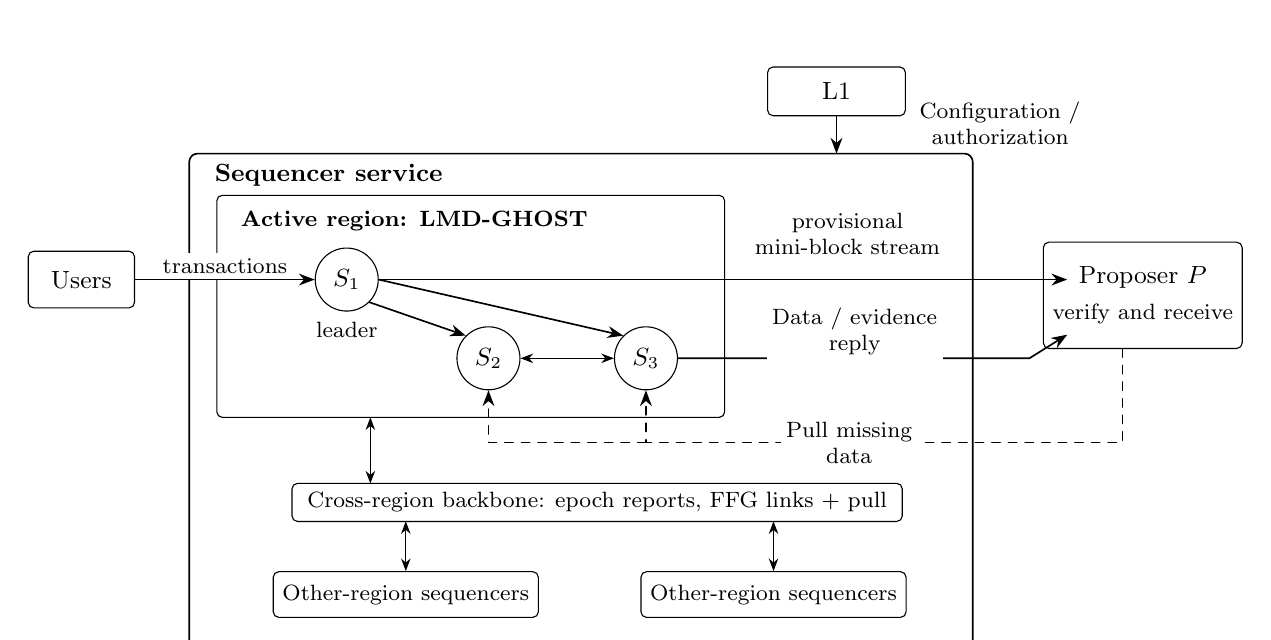
\begin{tikzpicture}[
  x=1cm,y=1cm,
  font=\small,
  line cap=round,line join=round,
  archbox/.style={draw,rounded corners=2pt,align=center,fill=white},
  archseq/.style={draw,circle,minimum size=8mm,inner sep=1pt,fill=white},
  archflow/.style={-{Stealth[length=2mm]},semithick},
  archpull/.style={-{Stealth[length=2mm]},semithick,dashed},
  archcontrol/.style={{Stealth[length=1.6mm]}-{Stealth[length=1.6mm]},thin},
  archlabel/.style={font=\footnotesize,fill=white,inner sep=2pt,align=center}
]
  % The outer box is the protocol boundary; P, users, and L1 are external.
  \draw[rounded corners=3pt,semithick] (2.25,-0.85) rectangle (12.20,5.45);
  \node[anchor=west,font=\small\bfseries] at (2.45,5.18) {Sequencer service};
  \draw[rounded corners=2pt] (2.60,2.10) rectangle (9.05,4.92);
  \node[anchor=north west,font=\footnotesize\bfseries] at (2.78,4.84)
    {Active region: LMD-GHOST};

  \node[archbox,minimum width=1.35cm,minimum height=.72cm] (users) at (.88,3.85)
    {Users};
  \node[archseq] (leader) at (4.25,3.85) {$S_1$};
  \node[archlabel,anchor=north] at (4.25,3.39) {leader};
  \node[archseq] (peerone) at (6.05,2.85) {$S_2$};
  \node[archseq] (peertwo) at (8.05,2.85) {$S_3$};
  \draw[archflow] (leader.south east) -- (peerone.north west);
  \draw[archflow] (leader.east) -- (peertwo.north west);
  \draw[archcontrol] (peerone.east) -- (peertwo.west);
  \draw[archflow] (users.east) -- node[archlabel,above] {transactions} (leader.west);

  \node[archbox,minimum width=1.90cm,minimum height=1.35cm] (consumer) at (14.36,3.65)
    {Proposer $P$\\[2pt]\footnotesize verify and receive};
  \draw[archflow] (leader.east) -- (13.40,3.85);
  \node[archlabel] at (10.61,4.43) {provisional\\mini-block stream};
  \draw[archpull] (14.10,2.97) -- (14.10,1.78) -- (8.05,1.78) -- (peertwo.south);
  \draw[archpull] (8.05,1.78) -- (6.05,1.78) -- (peerone.south);
  \node[archlabel] at (10.63,1.78) {Pull missing\\data};
  \draw[archflow] (peertwo.east) -- (12.92,2.85) -- (13.40,3.15);
  \node[archlabel] at (10.70,3.19) {Data / evidence\\reply};

  % Cross-region traffic is routed through a separate backbone lane.
  \node[archbox,minimum width=7.75cm,minimum height=.48cm] (backbone) at (7.43,1.02)
    {\footnotesize Cross-region backbone: epoch reports, FFG links + pull};
  \draw[archcontrol] (4.55,2.10) -- (4.55,1.26);
  \node[archbox,minimum width=2.50cm,minimum height=.58cm] (regiontwo) at (5.00,-.15)
    {\footnotesize Other-region sequencers};
  \node[archbox,minimum width=2.50cm,minimum height=.58cm] (regionthree) at (9.67,-.15)
    {\footnotesize Other-region sequencers};
  \draw[archcontrol] (5.00,.78) -- (regiontwo.north);
  \draw[archcontrol] (9.67,.78) -- (regionthree.north);

  \node[archbox,minimum width=1.75cm,minimum height=.62cm] (lone) at (10.47,6.24)
    {L1};
  \draw[archflow] (lone.south) -- (10.47,5.45);
  \node[archlabel,anchor=west] at (11.45,5.84) {Configuration /\\authorization};
\end{tikzpicture}

\caption{The sequencing service and its external interfaces. The three drawn
sequencers illustrate roles, not an $n=3,f=1$ fault model. $P$ is an external
proposer/consumer that verifies and consumes the stream.}
\label{fig:architecture}
\end{figure}

Regional members use latest-message subtree weights to choose which available
branch to extend. Ordinary HEAD messages are fork-choice inputs, not commit
votes. A consumer may replace its speculative suffix when its head changes,
including during a local producer change. There is no regional VOTE quorum,
DECIDED certificate, certified GAP, or per-batch agreement completion.

Global checkpoints select and retain a prefix on a slower timescale. We keep
the reference model's explicit synchronous agreement on epoch reports: it
makes the checkpoint target common even when regional heads disagree.
Adjacent FFG links justify and finalize checkpoints, including rotation
authorizations. This additional global agreement is part of the construction
and its cost; neither plain LMD-GHOST nor FFG is assumed to make arbitrary
reports converge. The design adapts the separation between fork choice and
finality in Gasper~\cite{gasper,ethfork,ffg}, rather than copying all of its
committee, fork-choice, or timing rules.

\section{System Model and Setup}\label{sec:model}
\subsection{Participants and L1 authorization}
The sequencers form a fixed set $V=\biguplus_{i=1}^{m}V_i$. Write
$S_{i,j}\in V_i$, $n_i=|V_i|$, $N=|V|$, and let $w_S>0$ be the voting weight
of $S$. For $U\subseteq V$, put
\[
 \wt(U)=\sum_{S\in U}w_S,\qquad W_i=\wt(V_i),\qquad W=\wt(V).
\]
A quorum of committee $Q$ has distinct signers of weight $>2\wt(Q)/3$.
Regional HEAD selection has no quorum threshold. Global FFG certificates and
regional readiness certificates use this threshold. Clients submit transaction
bytes to the current producer; $P$ is an external proposer consuming the stream.

L1 installs
\begin{equation}\label{eq:cfg}
 \Cfg_c=(c,V,\{V_i\},w,\mathcal L,\Theta,G_0).
\end{equation}
Here $c$ binds the chain and configuration; $\mathcal L$ gives a cyclic list
containing each member of each region once and a cyclic region list.
$\Theta$ fixes the slot duration $\tau_R$, slots per local term $N_R$,
global epoch duration $T_G$, geographic timers $N_G,K_G$, object limits,
retention and admission rules. $G_0$ supplies a justified and finalized
checkpoint, the initial region and the initial stream tip.
For clarity, regions use the same $\tau_R$ and $N_R$ in this reference.
Require $T_G/\tau_R$ to be a positive integer so that epoch boundaries are
also regional slot boundaries.

L1 authorizes local production by the clock schedule in
\cref{alg:localchange}; no local certificate is needed to move to the next
slot. A finalized control transition authorizes each new global view,
including a restart in the same region. Neither transition needs a new L1
transaction. Membership and weights stay fixed during the configuration.

\subsection{Cryptographic Primitives}
Nodes use authenticated point-to-point channels, transferable signatures
$\Sig_S(m)$ with verifier $\Ver_S(m,\sigma)$, and a binding hash $\Hash$. 
A quorum certificate $\QC_Q(m)$ contains distinct configured signers on the
same statement $m$ whose weight exceeds $2\wt(Q)/3$; the verifier checks all
of these conditions.

\subsection{Communication and time}\label{sec:network}
A common logical clock fixes slot and epoch boundaries. Complete admitted
objects between responsive honest nodes arrive, are retrieved and are verified
within $\Delta_R$ in a live region and $\Delta_G$ globally. 
A network backbone supports the cross-region data delivery.  $\Delta_G$ already includes the necessary
end-to-end route and verification time.
 Actual regional delay is
$\delta_R\leq\Delta_R$. The global budget also covers dissemination to healthy
regional participants before an anchor-installation boundary.

The communication between the sequencer service and the proposer has a delay bound  of $\Delta_P$.

\subsection{Honesty, availability, and retained data}
\begin{assumption}[Honest supermajorities]\label[assumption]{ass:env}
The Byzantine set $B$ is fixed during a configuration. For every region,
$\wt(V_i\setminus B)>2W_i/3$. Historical honest keys stay uncompromised.
\end{assumption}
Availability is separate from honesty. For global progress, an honest set
$H_G$ of weight $>2W/3$ remains responsive throughout the execution under
analysis. A healthy eligible region $i$ has
$\wt(H_G\cap V_i)>2W_i/3$ and regional delivery within $\Delta_R$ on that
set. It can be the current region after recovery. A merely honest but offline
member supplies neither timely votes nor timely data.



\subsection{Views, epochs, and block heights}\label{sec:indices}
A global view $\gv$ authorizes one region; its activation time is
$t_{\gv}$. A local view $\lv$ names a scheduled producer term within it.
The regional slot number $u$ increases with the clock, regardless of output.
\begin{table}[H]\centering\small
\begin{tabularx}{\textwidth}{@{}p{.15\textwidth}Y@{}}\toprule
Symbol & Meaning and update rule\\\midrule
$i$ & Region identity, not a round number.\\
$\gv$ & Global view; increases at finalized activation, even for same-region restart.\\
$\lv$ & Local view; $\lfloor(u-1)/N_R\rfloor$, reset on a new global view.\\
$u$ & Clock slot, starting at one; a missing slot needs no GAP record.\\
$e$ & Global epoch $[(e-1)T_G,eT_G)$; advances independently of production.\\
$h$ & Mini-block height along a branch; speculative forks can reuse a height.\\
\bottomrule\end{tabularx}
\caption{Region identity, authority, clock positions and stream positions.}
\end{table}
For example, $(\gv,\lv,i)=(4,0,2)$ may become $(4,1,2)$ at the next local
term boundary. A finalized handoff to region 3 gives $(5,0,3)$; a same-region
restart gives $(5,0,2)$. Neither changes the global epoch clock nor resets the
inherited stream height. Write $L\pre L'$ for the prefix relation on ordered
mini-block sequences.

\section{Service Specification}\label{sec:spec}
The consumer maintains a finalized log $L_P$ and a replaceable speculative
branch above its installed global anchor. The interface exports
\[
 \Tag{SetPreview}_P(\gv,h_0,q_{h_0},\beta),\qquad
 \Tag{Deliver}_P(h,M_h,\pi_G).
\]
SetPreview replaces the previous speculative suffix by the verified branch
$\beta$ above the named anchor. Its implementation reports the common ancestor,
retracted positions and new positions; a height alone does not identify an
entry. It is not an append-only output and is not a regional finality promise.
It may change during a local term, at a local rotation, when a global anchor
is installed, or at a geographic handoff. Empty $\beta$ is permitted.

A newly justified checkpoint fixes an \emph{adopted} prefix of the global
control chain. It becomes the regional fork-choice anchor at the next fixed
epoch boundary. Finalized checkpoints authorize append-only Deliver after
retrieval. The adopted anchor can therefore lie ahead of $L_P$; installing it
does not itself emit Deliver. These checkpoint-level properties do not give a
per-mini-block finality time or a promise to retain any particular preview.

\begin{definition}[Authorized stream with reorgable previews]\label{def:service}
Within the stated cryptographic and fault assumptions:
\begin{enumerate}[label=\textnormal{(\roman*)}]
\item Every accepted branch has complete, consecutively linked bytes signed
by the producers authorized for its slots. This verifies order and authority,
not EVM execution or transaction fairness.
\item Honest consumers' delivered logs are prefix-compatible, and each
$L_P(t)$ is a prefix of $L_P(t')$ for $t\leq t'$. A position is delivered once.
No corresponding agreement or monotonicity is required of SetPreview.
\item A valid finalized handoff preserves every globally adopted entry.
Current speculative data uses the current global view; old signatures remain
verifiable as historical evidence.
\item Under the global envelope, admitted workload and tenure conditions,
and an eventual healthy eligible region, adopted heights and finalized
delivery grow. A particular batch, preview or submitted transaction need not
survive. An empty transaction list may still form a new mini-block.
\end{enumerate}
\end{definition}
We measure proposal dissemination, preview update, global adoption and finalized
delivery separately. There is no regional decision latency. A finite set of
HEAD signatures authenticates those messages; it cannot prove that the
receiver has the latest message from every member or a globally canonical head.

\section{Protocol Objects and Interfaces}\label{sec:objects}
\subsection{Signed mini-blocks and batches}
Let a batch in slot $u$ contain $k$ mini-blocks, $1\leq k\leq b_R$, with
starting tip $(h_0,q_{h_0})$. For $1\leq j\leq k$, define
\begin{align}
 H_{h_0+j}&=(c,\gv,\lv,u,j,h_0+j,q_{h_0+j-1},
                    \Hash(\Tag{TXLIST},\mathcal X_{h_0+j})),\label{eq:block}\\
 q_{h_0+j}&=\Hash(\Tag{MINIBLOCK},H_{h_0+j}),\nonumber\\
 M_{h_0+j}&=(H_{h_0+j},\mathcal X_{h_0+j},
                \Sig_\ell(\Tag{ORDER},H_{h_0+j})).\nonumber
\end{align}
The ordered transaction list commitment includes length and multiplicity.
A batch envelope is
\begin{equation}\label{eq:proposal}
 x=(c,\gv,\lv,u,h_0,q_{h_0},k,q_{h_0+k}),\quad
 X=(x,M_{h_0+1},\ldots,M_{h_0+k},\Sig_\ell(\Tag{PROPOSE},x)).
\end{equation}
Its complete size is at most $B_R$. Batch identifiers are $\Hash(\Tag{BATCH},x)$;
fork-choice edges are complete batches and their tips are mini-block digests.
A one-mini-block batch gives mini-block granularity. Multiple-mini-block
batches are indivisible for fork choice and checkpoint packing.

\Proc{ValidBatch} verifies all commitments, signatures, size bounds,
the exact parent tip and consecutive heights, and $\ell=\ell(\gv,u)$ and
$\lv=\lfloor(u-1)/N_R\rfloor$ from the activation and schedule.
Between batches in one global view, producer slot numbers strictly increase;
several mini-blocks within one batch share its slot. A branch in a new global
view starts from the inherited tip, which may belong to an older view.
Changing leader does not change the signatures on inherited batches.

A valid branch relative to an adopted tip $\alpha=(h,q)$ is a complete list
of such batches extending $q$, all new batches in the effective global view.
The first slot exceeds the anchor batch's slot when that batch is in the same
global view. Validity does not require a producer to prove its private LMD
view; honest production follows LMD, while Byzantine choices of a valid parent
remain admissible forks.

\subsection{HEAD messages and eligible trees}\label{sec:headobjects}
A regional member signs at most one
\[
 a_{S,u}=\Sig_S(\Tag{HEAD},c,\gv,u,q)
\]
per slot of the active global view. The tip $q$ is either the installed anchor
or a complete available branch whose last slot is at most $u$.
Nodes reject future-slot HEAD messages for current processing; historical
messages may be retained as evidence. Only members of the active region
contribute regional HEAD weight.

At node $p$, $\mathcal T_p$ is the finite tree of admitted complete branches
extending its installed anchor. Missing bodies, invalid signatures and branches
incompatible with that anchor are ineligible. The configuration bounds the
eligible speculative depth by $d_R\geq1$ complete batches. A full branch at
that depth may be previewed and reported, but cannot be extended until anchor
advancement frees space. The data/verification budget covers a path of this
depth. Nodes admit at most two candidate batches per producer slot for local
fork choice, retain conflict evidence, and reserve capacity for prescribed
honest traffic. Global report validation is independent of which candidates
a particular node admitted locally.

For each signer, maintain its largest observed authenticated HEAD slot and
all distinct tip values at that slot (capped at two for conflict detection).
A strictly newer slot replaces the old record. Two tips at the latest slot
give that signer zero weight until a newer unambiguous slot is observed.
A latest message with missing data or an incompatible branch also gives zero
weight; it does not resurrect an older vote. Fetching its data can make the
same latest record eligible. This bookkeeping is not an authority change.

\subsection{Global checkpoints, reports, and anchors}\label{sec:gobjects}
The global state is
\[
 S=(\gv,i,A,t_{\gv},h,q,z,e_{\gv},p),
\]
where $A$ is the activation proof, $(h,q)$ the adopted tip, $z$ the number of
consecutive epochs without adopted-height growth, $e_{\gv}$ the activation
epoch, and $p$ an optional pending rotation. Genesis supplies these fields.
The checkpoint at epoch $e$ is
\begin{equation}\label{eq:global}
 C_e=(c,e,g_{e-1},\mu,S_e,\Hash(\mathbf r_e)),\qquad
 g_e=\Hash(\Tag{CHECKPOINT},C_e),
\end{equation}
with $\mu\in\{\Tag{ADVANCE},\Tag{HOLD},\Tag{ROTATE},\Tag{CONFIRM}\}$.
Even HOLD has a new epoch and a new checkpoint identity.

At the start of epoch $e$, install the justified parent $C_{e-1}$ and any
finalized activation due at that boundary. Call the resulting state effective.
A signed report from $S\in V_j$ is
\[
 r_{S,e}=(c,e,g_{e-1},A_e,\beta_{S,e},q_{S,e},\mathsf{ready}),
\]
where $A_e$ supplies the already existing proof of any activation just applied.
If $j=i$, $\beta_{S,e}$ is a complete branch from the effective adopted tip,
and $q_{S,e}$ is exactly its endpoint. It has at most $b_G$ whole batches and
$B_G$ relative bytes. All its producer slots end no later than the epoch's
start. For $j\ne i$, the branch must be empty. An empty branch endorses the
effective anchor. The signed active-region report is one fresh checkpoint
snapshot endorsement, weighted once by its origin. It does not assert that
other members have seen that head, and need not reproduce their HEAD messages.

For the report snapshot, put
\[
 \bar u_e=\left\lfloor\frac{(e-1)T_G-t_{\gv}}{\tau_R}\right\rfloor.
\]
After installing the effective anchor, first filter the candidate tree to
batches with slots at most $\bar u_e$, and then run LMD on that filtered tree.
Latest-HEAD records whose vote slots exceed $\bar u_e$ contribute zero to
this snapshot; no older record is revived. Pending objects for the slot just
starting are excluded even if their bytes arrived early. At activation
$\bar u_e=0$, so the new global view's first report has an empty branch.

An honest active member reports the longest fitting complete prefix of this
cutoff-filtered LMD path. If that path is nonempty, the admitted prefix must
be nonempty. In particular, $b_G,B_G$ must
fit one entire legal batch and its relative authorization evidence. A truncated
report endorses its admitted endpoint, not the unreported original head.
Inactive members do not influence regional fork-choice weight.

A true READY promises possession and retention of the parent's entire adopted
prefix and evidence, and readiness to start global view $\gv+1$ in the signer's
configured region. It binds $(c,e,g_{e-1},\gv+1,j,h,q)$ after any activation.
Every healthy eligible honest member with these objects sets READY true,
even if it reports no extension. Readiness is recollected for each parent.

\Proc{ValidReport} checks the origin, epoch, parent, activation, complete
relative branch, slot cutoff, current global view, reported endpoint and size
limits. Byzantine reports can endorse any valid branch and lie about readiness;
a regional ready quorum still contains honest holders. Different reports may
contain incompatible branches. A verifier accepts report bodies independently
of its local speculative candidate cap and retains their bytes.

\Proc{ValidCheckpoint} checks every non-bottom report, its vector commitment,
and the exact deterministic state transition. A report vector alone is not a
portable agreement proof; the global FFG certificate endorses the derived
checkpoint. Missing control ancestry or bytes must be obtained before use.

\subsection{Data transport and persistent state}\label{sec:transport}
Transport uses authenticated ANNOUNCE, GET and DATA messages. An object ID
binds its type, producer or checkpoint digest, and exact branch/range; it is
not merely a height interval. A supplier need not be the producer.
Receivers verify complete contents and original evidence, cache by digest,
and request only missing bodies. Late or conflicting data is never resolved
by overwriting a height-indexed cache entry.

Sequencers persist the configuration, activation history, verified global
chain and links, retained data, and signing history. Regional state includes
the installed anchor, candidate tree and latest-HEAD records. Consumers
add their delivered log, speculative branch and missing-object set. An anchor
update preserves signing watermarks; a fresh global view uses new domains.

\Needspace{17\baselineskip}
\section{The Protocol}\label{sec:protocol}
\subsection{Clock-driven local rotation}\label{sec:localchange}
\begin{protocol}{alg:localchange}{Local authority independent of slot success}
For global view $\gv$ activated at $t_{\gv}$ in region $i$, slot $u\geq1$
starts at $t_{\gv,u}=t_{\gv}+(u-1)\tau_R$. Define
\[
 \lv(u)=\left\lfloor\frac{u-1}{N_R}\right\rfloor,\qquad
 \ell(\gv,u)=\mathcal L_i[\lv(u)\bmod n_i].
\]
\begin{enumerate}[label=\textbf{L\arabic*.}]
\item At every slot boundary, derive the authorized producer from the clock,
configuration and activation proof. The first member of the list starts a new
global view. A silent slot creates no record and changes no parent hash.
\item At a term boundary, the next producer starts from its own eligible LMD
head above the installed anchor. It needs no release signature from its
predecessor, no local quorum, and no certified outcome for the missing slots.
\item A recovering node restores its signing history, activation and current
anchor, retrieves missing objects and joins a future slot. It does not sign
retroactively for expired slots. A private timeout triggers retrieval, not an
unscheduled authority change.
\end{enumerate}
\end{protocol}
The former $K_R$ failure-streak rule is not used. A continuously unproductive
producer loses its term within $N_R$ slots, whether or not any observer can
prove why it failed. Early replacement would require an additional common
authorization rule and is outside this reference. Global view changes still
use the finalized protocol below.

\subsection{Regional production and LMD fork choice}\label{sec:regional}
\begin{protocol}{alg:head}{LMD-GHOST over a node's available regional tree}
\textbf{Input:} installed anchor $\alpha$, complete eligible tree $\mathcal T$,
latest usable HEAD tip $q_S$ for each regional member (if any).
For a child batch-tip $b$, put
\[
 \omega(b)=\sum_{S:\,q_S\text{ lies in the subtree rooted at }b}w_S.
\]
Start at $\alpha$. While the current node has eligible children, choose the
child with largest $\omega$, breaking ties by largest canonical batch digest.
Continue even when all child weights are zero. Return the reached tip and its
complete path. Recompute after eligible data, latest-message, or anchor updates.
\end{protocol}

\begin{protocol}{alg:regional}{One streaming slot, without a decision quorum}
\textbf{Participants:} active $V_i$; producer $\ell(\gv,u)$.
Choose $\tau_R>2\Delta_R$; all epoch boundaries are slot boundaries.
\begin{enumerate}[label=\textbf{R\arabic*.}]
\item \textbf{At slot start.} First install any boundary-due global anchor or
activation. A synchronized honest producer computes \Proc{Head}. If its
selected path has fewer than $d_R$ batches, it constructs one eligible batch
extending that tip, signs ORDER and PROPOSE, sends the complete object to the
region and pushes it to subscribed consumers. It may use empty transaction
lists. It signs at most one batch for this slot.
\item \textbf{On data.} Verify the complete batch and ancestry, slot authority
and admission bounds before adding it to the local tree. Buffer future-slot
objects without selecting or voting for them. Retain incompatible valid
historical objects as evidence, not as children of the current anchor.
\item \textbf{At }$t_{\gv,u}+\Delta_R$. Each synchronized member computes its
current head and signs one HEAD for slot $u$, including when the producer was
silent. Broadcast it to regional members. The head may be the anchor or a
branch produced in an earlier slot. Process received HEAD messages by
\cref{sec:headobjects}; no quorum is awaited.
\item \textbf{Continue.} Update the speculative head and serve data. At the
next clock boundary move to slot $u+1$, even if this slot had no proposal or
the members selected different heads. Global epoch processing runs in parallel.
\end{enumerate}
\end{protocol}

The $\Delta_R$ attestation point is a reference timing choice, not an internal
commit deadline. HEAD is chosen by fork choice rather than automatically voting
for the first received proposal. Producer push can expose data sooner.
LMD does not certify agreement on local heads: selective release of valid
branches or votes can make local views differ. Our progress proof below does
not require such heads to converge or each honest proposal to survive.

\begin{example}[A missed slot and a local reorganization]
The installed anchor is 100. Slot 7's producer is silent; slot 8 proceeds
without a GAP certificate. Its producer may extend 100 with 101--105.
If available HEAD weights later favor another authorized branch
101'--103', a node can replace its speculative suffix by that branch.
The two branches need not be prefix-compatible. Neither change modifies a
delivered entry. A subsequent global checkpoint may select either available
branch by its common report snapshot.
\end{example}

\Needspace{25\baselineskip}
\subsection{Push, repair, and consumer reorganization}\label{sec:pull}
\begin{protocol}{alg:pull}{Authenticated transport and separate output levels}
\begin{enumerate}[label=\textbf{D\arabic*.}]
\item \textbf{Push/announce.} Producers push each new batch once per subscriber.
Holders announce available heads and new global certificates every $T_A$ and
on relevant updates. An announcement is a retrieval hint, not confirmation.
\item \textbf{Repair.} Request the exact missing branch objects from regional
holders in configured order, with deadline $\theta_R$ per bounded attempt.
For adopted data also try global holders with deadline $\theta_G$. Validate
complete replies; cache by digest and avoid concurrent duplicate requests.
After exhausting a list, retry after $T_A$. Missing predecessors prevent output.
\item \textbf{SetPreview.} Verify activation, clock authority and complete
branch data. Select by the consumer's available LMD inputs, or label a
provider's selected branch as advisory. Replace only the speculative suffix,
reporting its common ancestor and withdrawals. Never label HEAD support as a
finality certificate. No preview branch may conflict with the installed anchor.
\item \textbf{Install an anchor.} Verify an extending global control proof.
At its specified epoch boundary install the adopted tip, obtain its complete
prefix, and discard incompatible candidate branches from fork choice.
Recompute the preview. Preserve all delivered entries. If proof or bytes are
missing, pause current-authority output until synchronization; a stale node's
view is not a new authorization. Do not roll back to a replayed ancestor proof.
\item \textbf{Deliver.} For a verified finalized checkpoint, retrieve and
validate its complete newly covered prefix, producer authority history and
finality links. Before appending, install its already-due anchor and all
intervening due activations, unless a newer extending anchor is installed.
Queue a proof whose required boundary has not arrived. Maintain the invariant
that the installed anchor's prefix contains the entire delivered log; prune
and recompute any conflicting preview before further output.
Append only previously undelivered positions in order. Delivery
does not require a regional certificate. Apply all intervening activations
in verified ancestry order during catch-up; old preview entries are identified
by digest and view, not reused height alone.
\end{enumerate}
\end{protocol}

Every justified checkpoint produced in epoch $e$ is installed for regional
production at the start of epoch $e+1$, after certificate dissemination. Its
adopted tip is the reorg floor, even before that checkpoint is finalized.
This is justified by the unique global control chain in this construction;
it is not a per-batch finality claim. A member missing that boundary's required
checkpoint does not originate a new batch, HEAD, or report from a stale anchor.
Clock slots still pass while it catches up. An old producer isolated from
global control can show stale previews to stale clients, but cannot extend the
new accepted control history after replacement.

\begin{figure}[htbp]\centering
% Native TikZ input. Requires \usepackage{tikz} and \usetikzlibrary{arrows.meta}.
% The panels show protocol dependencies, not equal-duration message rounds.
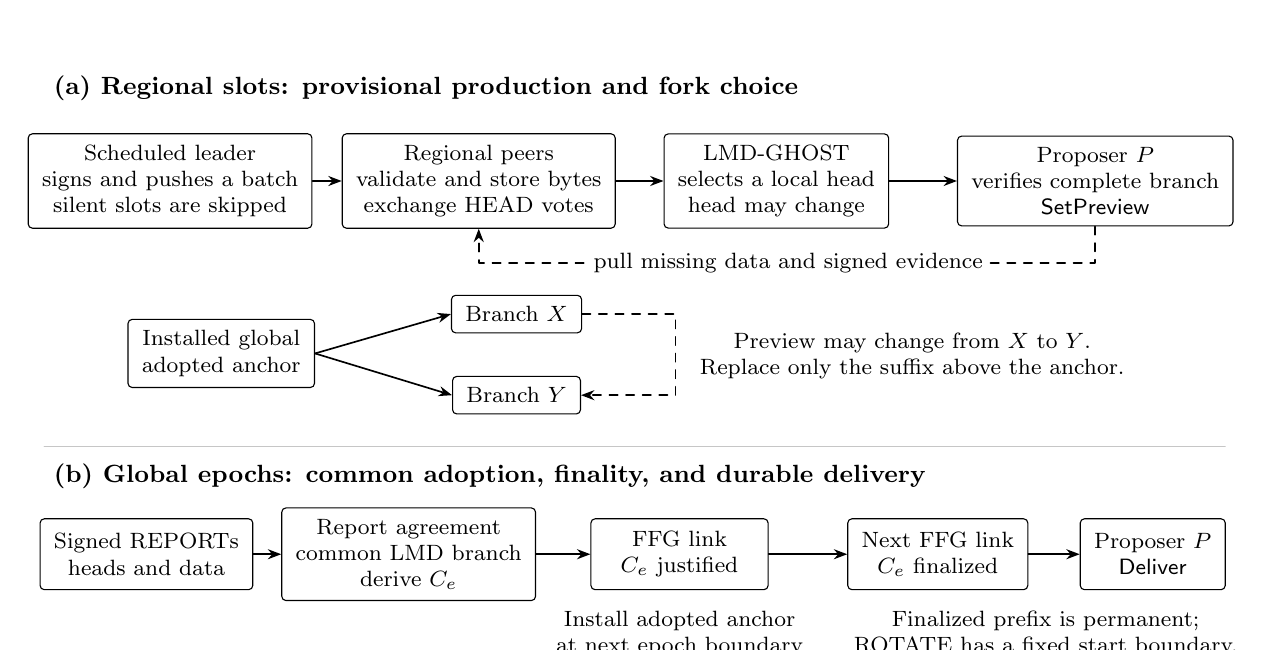
\begin{tikzpicture}[
  x=1cm,y=1cm,
  font=\small,
  line cap=round,line join=round,
  pipebox/.style={draw,rounded corners=1.5pt,fill=white,align=center,
    inner xsep=5pt,inner ysep=4pt,font=\footnotesize},
  pipeflow/.style={-{Stealth[length=1.7mm]},semithick},
  pipepull/.style={-{Stealth[length=1.7mm]},semithick,dashed},
  pipelabel/.style={font=\footnotesize,fill=white,inner sep=1.5pt,align=center}
]
  \node[anchor=west,font=\small\bfseries] at (0,6.90)
    {(a) Regional slots: provisional production and fork choice};
  \node[pipebox,minimum width=2.75cm,minimum height=1.10cm] (leader) at (1.60,5.72)
    {Scheduled leader\\signs and pushes a batch\\silent slots are skipped};
  \node[pipebox,minimum width=2.60cm,minimum height=1.10cm] (peers) at (5.52,5.72)
    {Regional peers\\validate and store bytes\\exchange HEAD votes};
  \node[pipebox,minimum width=2.40cm,minimum height=1.10cm] (head) at (9.30,5.72)
    {LMD-GHOST\\selects a local head\\head may change};
  \node[pipebox,minimum width=2.70cm,minimum height=1.10cm] (consumer) at (13.35,5.72)
    {Proposer $P$\\verifies complete branch\\$\mathsf{SetPreview}$};
  \draw[pipeflow] (leader.east) -- (peers.west);
  \draw[pipeflow] (peers.east) -- (head.west);
  \draw[pipeflow] (head.east) -- (consumer.west);
  \draw[pipepull] (consumer.south) -- (13.35,4.68) -- (5.52,4.68) -- (peers.south);
  \node[pipelabel] at (9.45,4.68) {pull missing data and signed evidence};

  \node[pipebox] (anchor) at (2.25,3.53) {Installed global\\adopted anchor};
  \node[pipebox] (branchx) at (6.00,4.03) {Branch $X$};
  \node[pipebox] (branchy) at (6.00,3.00) {Branch $Y$};
  \draw[pipeflow] (anchor.east) -- (branchx.west);
  \draw[pipeflow] (anchor.east) -- (branchy.west);
  \draw[pipepull] (branchx.east) -- (8.02,4.03) -- (8.02,3.00) -- (branchy.east);
  \node[pipelabel,anchor=west] at (8.27,3.50)
    {Preview may change from $X$ to $Y$.\\Replace only the suffix above the anchor.};

  \draw[gray!45] (0,2.35) -- (15.00,2.35);
  \node[anchor=west,font=\small\bfseries] at (0,1.97)
    {(b) Global epochs: common adoption, finality, and durable delivery};
  \node[pipebox,minimum width=2.00cm,minimum height=.90cm] (reports) at (1.30,.98)
    {Signed REPORTs\\heads and data};
  \node[pipebox,minimum width=2.65cm,minimum height=.90cm] (agreement) at (4.63,.98)
    {Report agreement\\common LMD branch\\derive $C_e$};
  \node[pipebox,minimum width=2.25cm,minimum height=.90cm] (justified) at (8.07,.98)
    {FFG link\\$C_e$ justified};
  \node[pipebox,minimum width=2.25cm,minimum height=.90cm] (finalized) at (11.35,.98)
    {Next FFG link\\$C_e$ finalized};
  \node[pipebox,minimum width=1.50cm,minimum height=.90cm] (deliver) at (14.08,.98)
    {Proposer $P$\\$\mathsf{Deliver}$};
  \draw[pipeflow] (reports.east) -- (agreement.west);
  \draw[pipeflow] (agreement.east) -- (justified.west);
  \draw[pipeflow] (justified.east) -- (finalized.west);
  \draw[pipeflow] (finalized.east) -- (deliver.west);
  \node[pipelabel,anchor=north] at (8.07,.32)
    {Install adopted anchor\\at next epoch boundary};
  \node[pipelabel,anchor=north] at (12.72,.32)
    {Finalized prefix is permanent;\\ROTATE has a fixed start boundary.};
\end{tikzpicture}

\caption{Regional production and HEAD messages support reorgable previews.
The separate epoch protocol selects an adopted prefix; an adjacent FFG link
finalizes the preceding checkpoint. No per-batch agreement completion gates
the regional stream.}
\label{fig:stream}
\end{figure}

\subsection{Epoch reports and checkpoint selection}\label{sec:global}
All $V$ participate in global epochs, regardless of which region produces.
The report cutoff is the epoch start; proposed batches in the new slot at that
boundary are for a later snapshot. Signatures bind reports to the exact parent,
so a delayed report for an earlier epoch cannot be counted again.

\begin{protocol}{alg:global}{Global report agreement and one FFG link}
\textbf{Common initial state:} justified $C_{e-1}$, complete adopted data,
and previous finality proofs. $C_0$ is justified and finalized.
\begin{enumerate}[label=\textbf{G\arabic*.}]
\item \textbf{At epoch start.} Install the parent and any due activation.
Active-region members re-root local trees, apply the completed-slot cutoff
in \cref{sec:gobjects}, and only then run the snapshot fork choice.
Originate the report prescribed there; READY depends on possession of the
parent prefix, not on whether any new batch exists. Local production in the
new slot then proceeds independently.
\item \textbf{Agree on reports.} Run $N$ parallel authenticated broadcasts
of \cref{alg:ab}, one per origin, with domain $(\Tag{REPORT},c,e,g_{e-1})$,
round length $\Delta_G$, and predicate \Proc{ValidReport}. After $N\Delta_G$
every responsive honest member has the same vector $\mathbf r_e$ of reports
or $\botv$. Missing/ambiguous origins become $\botv$.
\item \textbf{Derive and vote.} Compute \cref{alg:gtransition} on that vector,
retain complete selected data, and construct $C_e$. With justified source
$C_{e-1}$, sign $(\Tag{FFG},c,e-1,g_{e-1},e,g_e)$ subject to
\cref{alg:finality}, and disseminate it globally.
\item \textbf{Export.} Form the global link quorum by $(N+1)\Delta_G$ and
disseminate its certificate by $(N+2)\Delta_G$. Notify consumers and holders.
Require $T_G\geq(N+3)\Delta_G$; the remaining margin supplies the next
boundary's anchor, data and activation proof. Do not install $C_e$ for
regional production before that fixed boundary.
\end{enumerate}
\end{protocol}

\begin{protocol}{alg:gtransition}{Common LMD snapshot and region selection}
\textbf{Input:} effective parent state with adopted tip $\alpha=(h,q)$,
and common vector $\mathbf r_e$.
\begin{enumerate}[label=\textbf{T\arabic*.}]
\item \textbf{Pending rotation.} If a rotation remains pending and is not yet
activated, output CONFIRM with the same adopted tip, active region and pending
package. Adopt no new regional data in this step.
\item \textbf{Snapshot tree.} Otherwise form the union $\mathcal T_e$ of all
valid active-region report paths, rooted at $\alpha$. Each non-bottom active
origin contributes $w_S$ once to its reported endpoint. Run \Proc{Head} on
this common tree and these fresh snapshot votes, with the same digest tie rule.
Let the chosen tip be $(h^+,q^+)$; an empty tree chooses $\alpha$.
Set $z^+=0$ if $h^+>h$, and $z^+=z+1$ otherwise.
\item \textbf{Readiness and trigger.} Region $j$ is ready when true READY
reports bound to this parent have weight $>2W_j/3$. A switch is due if
$e-e_{\gv}\geq N_G$ or $z^+\geq K_G$. If due and another region is ready,
choose the first such region after $i$ in the cyclic region list. Otherwise,
if $z^+\geq K_G$, no other region is ready and $i$ is ready, choose $j=i$.
\item \textbf{Rotate or adopt.} If a successor was chosen, output ROTATE and
retain the \emph{parent} tip $(h,q)$, storing
\[
 p=(\gv+1,j,h,q,e,\mathsf{readyProof},\mathsf{reason}).
\]
No new range is adopted: the readiness proof refers to the parent tip.
Otherwise adopt $(h^+,q^+)$, set $z=z^+$, and output ADVANCE if the height
grew or HOLD otherwise. Without a ready successor, current service can continue.
\end{enumerate}
\end{protocol}

The snapshot rule is not a longest-chain rule and does not assume regional
branches are compatible. It uses a fresh per-origin REPORT endorsement rather
than all ordinary HEAD histories. An equivocating REPORT origin has one common
AB output, possibly bottom, and cannot have its weight counted twice.
The union has at most $Nb_G$ batch entries before deduplication, not merely
$b_G$. The selected path is a prefix of some reported path, so it still fits
one report's branch limits. Report agreement already makes the control target
unique under synchrony; FFG supplies the checkpoint finality and activation
discipline. Removing this epoch-level agreement would be a separate redesign.

\subsection{Finality and geographic activation}\label{sec:finality}
\begin{protocol}{alg:finality}{Adjacent FFG links and fixed activation}
\begin{enumerate}[label=\textbf{F\arabic*.}]
\item \textbf{Vote.} Check the complete deterministic target and justified
parent. Persist at most one FFG statement per target epoch. Never sign
surrounding links with $s_1<s_2<t_2<t_1$, or a target conflicting with the
known finalized control prefix. This construction uses only links $(e-1,e)$.
\item \textbf{Justify/finalize.} A link $C_s\Rightarrow C_t$ includes
$\QC_V(\Tag{FFG},c,s,g_s,t,g_t)$ and matching ancestry, with $s<t$ and a
justified source. It justifies the target. A justified $C_e$ is finalized by a
link to its direct child $C_{e+1}$; ancestors are finalized as well.
Verification starts from a trusted control anchor, not from an isolated root.
\item \textbf{Activate.} If ROTATE at $C_r$ is finalized by
$C_r\Rightarrow C_{r+1}$, activate its successor at the beginning of epoch
$r+2$, time $(r+1)T_G$. Before then it obtains and verifies the proof and
retained data. Missing objects prevent that node from starting.
\item \textbf{Initialize.} At this boundary apply the proof to the strict
ancestor ROTATE: increment $\gv$, set the named region, $t_{\gv}=(r+1)T_G$,
$\lv=0$, $u=1$, $z=0$, $e_{\gv}=r+2$, clear $p$, and retain $(h,q)$.
Use the region's configured first producer and a fresh HEAD domain. Existing
checkpoints and signing histories are unchanged. The new target records this
pre-transition activation before applying \cref{alg:gtransition}.
\end{enumerate}
\end{protocol}

A ready quorum proves possession when signed, not continued availability.
If the selected region fails before activation, epochs still advance and
eventually select another ready region. A same-region restart uses exactly
the same READY, ROTATE, CONFIRM and activation rules. Neither path waits for
any local slot to finish or for a failed producer to acknowledge handoff.

\begin{example}[Checkpoint selection and geographic recovery]
The adopted tip is 100; some members preview 101--110 while others preview
101'--106'. Global reports may contain both branches. The common snapshot
selects one, say the second, and ADVANCE adopts 106'. At the next boundary all
current producers re-root there; old speculative 101--110 may be withdrawn.
If a ROTATE instead takes precedence, its retained tip remains 100 and both
tails are unretained. CONFIRM finalizes the rotation; the successor starts
from 100. Once a prefix has been globally adopted, every later handoff retains
it even if it was not yet finalized when the outage began.
\end{example}

\subsection{Equivocation evidence}\label{sec:evidence}
\begin{protocol}{alg:evidence}{Authenticated conflicts and their scope}
Verify both signatures before ordinary conflict discard. Two different
semantic statements by one configured signer give evidence in these domains:
\begin{itemize}
\item PROPOSE: equal $(c,\gv,u)$ but different batch envelopes;
\item ORDER: equal $(c,\gv,u,j)$ but different mini-block headers;
\item HEAD: equal $(c,\gv,u)$ but different tips;
\item REPORT: equal $(c,e,g_{e-1},S)$ but different reports;
\item FFG: equal target epoch but different link statements, or a surround pair.
\end{itemize}
Retain and forward at most one evidence pair per signer/type/domain. Apply
the local latest-HEAD exclusion rule; do not change configured quorum weights
or retroactively recompute an already certified global checkpoint.
\end{protocol}
Different-slot HEAD choices, local reorgs, silence, missing DATA and forwarding
conflicting origin values in the global AB protocol are not these offenses.
Old-view statements can remain evidence without being eligible current data.
Financial penalties and adjudication lie outside the service.

\section{Correctness and Soundness}\label{sec:proofs}
All statements use the fixed configuration, cryptographic assumptions and
explicit availability bounds above. A certificate safety claim is distinct
from a claim that a certificate will be formed. No result asserts agreement
of speculative regional heads.

\begin{lemma}[Quorum intersection]\label[lemma]{lem:intersection}
Two quorums of a committee of weight $W_Q$ share weight $>W_Q/3$, hence an
honest signer when Byzantine weight is $<W_Q/3$.
\end{lemma}
\begin{proof}
For signer sets $U,U'$, inclusion--exclusion gives
$\wt(U\cap U')\geq\wt(U)+\wt(U')-W_Q>W_Q/3$.
\end{proof}

\begin{lemma}[Clock authority and valid branches]\label[lemma]{lem:authority}
For a fixed activation, exactly one configured producer is authorized in each
slot. Slot and local-view advancement do not depend on a previous slot's
messages. Every branch accepted by \Proc{ValidBatch} has the claimed contents,
order and slot-authorized signatures. Equivocation can yield multiple valid
branches; this lemma does not exclude it.
\end{lemma}
\begin{proof}
The activation fixes $t_{\gv}$ and the region. The formulas in
\cref{alg:localchange} determine $u$, $\lv(u)$ and a unique list entry.
They advance even when no batch exists. Signature unforgeability authenticates
the producer for each header and envelope. Hash binding and consecutive parent
checks fix the ordered bytes by induction along a branch. Strictly increasing
inter-batch slots prohibit cycles, while a local producer change leaves old
signatures intact. A Byzantine authorized producer can sign two envelopes;
validity and evidence detection deliberately do not make them one branch.
\end{proof}

\begin{lemma}[Deterministic fork choice, without local agreement]
\label[lemma]{lem:head}
Given the same finite eligible tree and latest-message map, \Proc{Head}
returns the same available path. Its result extends its input anchor. If the
tree has a child of the anchor, the result is a nonempty extension.
Different local inputs need not yield compatible results.
\end{lemma}
\begin{proof}
Each node's child set has a unique maximizing pair (weight, canonical digest).
Each step descends in a finite acyclic tree and thus terminates at a leaf.
The rule descends even through a zero-weight tie, establishing the last
positive claim without a quorum premise. Missing-data and same-slot-conflict
exclusions are local functions of the map; they need not be identical at
different receivers. A two-child root with opposing local weight maps gives
different selected branches, so no prefix-agreement conclusion follows.
\end{proof}

\begin{lemma}[Authenticated origin broadcast]\label[lemma]{lem:ab}
In \cref{alg:ab}, all responsive honest members return the same value or
bottom. An honest responsive origin's valid input is returned. Every non-bottom
output has a complete valid witness. The protocol terminates in $n$ rounds,
under its complete-object delivery bound, if at least one member is honest
and responsive.
\end{lemma}
\begin{proof}
Consider a value retained by an honest responsive member in round $r$.
If its chain contains an honest responsive signer at position $k$, that
signer already multicast its prefix in round $k$. All responsive honest
receivers then either retained the value or already held two values.
If no chain signer is honest and responsive, its length is at most $n-1$;
the receiving member appends its signature and forwards next round, unless
it already forwarded that value. Its earlier multicast suffices in that case.
A length-$n$ chain contains an honest responsive member.

Thus, by round $n$, any honestly retained value is retained by every honest
responsive member or encounters a set that already has two values. If one
member has two values, apply this fact to both: all end with two and return
bottom. Otherwise every nonempty honest set contains the same sole value.
If all sets are empty, all return bottom. An honest origin signs one value;
first-round delivery and unforgeability give honest-origin validity. Witness
checks give external validity. The fixed deadlines give termination. Sets
containing two values need not contain the same pair when the origin equivocates
three or more ways; only the common bottom output is needed.
\end{proof}

\begin{lemma}[Common checkpoint selection from conflicting reports]
\label[lemma]{lem:snapshot}
For a common effective parent and common report vector, the transition yields
one target and its adopted branch extends the parent. If no rotation is pending
or selected and at least one valid active report has a nonempty branch, the
adopted height strictly increases. The selected path fits one report's branch
limits even though verifying the union can cost $NB_G$ bytes.
\end{lemma}
\begin{proof}
Each admitted branch starts at the same anchor. Deduplicating shared prefixes
therefore gives a finite rooted tree, not necessarily one chain. Each origin
contributes one fixed weight to its endpoint. \Cref{lem:head} supplies a unique
path and chooses a nonempty extension when a child exists. A selected leaf
is the endpoint of a reported path; its entire root-to-leaf path was included
in that report. Thus selection respects that report's limits. Readiness,
timers and cyclic successor choice are also deterministic. HOLD and CONFIRM
preserve the parent, and ROTATE explicitly retains the parent instead of the
candidate extension. All possible transitions are therefore prefix-preserving.
\end{proof}

\begin{theorem}[Global agreement, finality, and authority]\label[theorem]{thm:global}
Under the global envelope and epoch budget, all responsive honest global
members derive and justify the same $C_e$ and finalize $C_{e-1}$ in each epoch.
Adopted prefixes are monotone. A finalized ROTATE gives one successor global
view at its fixed boundary and preserves all previously adopted data.
Conflicting globally certified checkpoints at the same epoch cannot both
exist under the signing and Byzantine-weight assumptions.
\end{theorem}
\begin{proof}
Induct from genesis. The prior certificate phase supplies the parent, adopted
bytes and due activation proof before the next boundary. These make the
effective state and report-validity predicate common. \Cref{lem:ab} yields
the same report vector; \cref{lem:snapshot} yields the same target and complete
selected prefix. All responsive honest members retain those bytes and vote.
Their weight exceeds $2W/3$, so the link is formed and disseminated within
the budget. Source and target epochs increase together; these adjacent links
obey the honest double-vote and surround constraints. The target is justified
and its direct parent finalized.

Every transition extends or retains the parent prefix. Installation occurs at
a common future boundary, so production and the next snapshot use the same
certified anchor when they are healthy. A pending successor is consumed only
through the finality proof of its ancestor ROTATE; activation does not alter
either existing checkpoint. It resets the slot/signing domains using $\gv+1$
and preserves the inherited tip. This applies equally to same-region restart.
Finally, two different certificates for one target epoch would intersect in an
honest signer that signed two targets, contradicting its persistent rule.
Since all accepted checkpoints link to the immediately preceding epoch,
induction also rules out conflicting certified control histories.
\end{proof}

The proof uses explicit global report agreement; it is not a claim that FFG
alone chooses a common target. The finality rule is the adjacent-link
Casper-FFG pattern on this control chain. It does not implement every Gasper
justification case, dynamic validator set, or partial-synchrony recovery rule.

\begin{theorem}[Consumer verification and delivered-prefix safety]
\label[theorem]{thm:sound}
\Cref{alg:pull} preserves valid previews and append-only, prefix-compatible
delivered logs. Local reorgs and global handoffs cannot remove a delivered
entry. No correctness statement about EVM execution follows.
\end{theorem}
\begin{proof}
\Cref{lem:authority} authenticates each candidate's ordered data and producer
history. \Cref{thm:global} supplies a single control history with monotone
adopted prefixes, hence compatible finalized prefixes. A consumer retrieves
and verifies all new data before appending each undelivered position exactly
once. Its delivered log is therefore a prefix of this single finalized stream.
Changing data, order, parent, slot or producer breaks a verified commitment,
signature or authority rule.

SetPreview can replace a suffix, but only above the installed anchor, which
extends every earlier delivered prefix. When a newer proof is learned, applying
its intervening activations and anchor transitions before current output
prevents old-view reuse of a height from being mistaken for retained data.
Replay cannot decrease the consumer's control anchor. Missing proof or bytes
pauses output rather than fabricating a prefix. None of these checks evaluate
execution state, receipts, transaction selection or publication by $P$.
\end{proof}

\begin{lemma}[Retention and repair]\label[lemma]{lem:pull}
A globally justified checkpoint has responsive honest holders of its complete
adopted prefix under the global envelope. If a bounded requested object has
$a$ failed attempts before a responsive honest holder, its repair time after
the first request is at most $(a+1)\theta$. A speculative object's availability
requires an actual reachable holder; its signature or HEAD alone is not such
a guarantee to a receiver.
\end{lemma}
\begin{proof}
The responsive honest global members retain the complete selected prefix
before voting and keep it for the configuration. Each failed attempt costs at
most $\theta$, and the next admitted honest response verifies within that
deadline. The producer and supplier may differ because the original evidence
is checked. A speculative batch held only by an unavailable Byzantine producer
has no analogous retention guarantee; the conditional statement does not
apply to it.
\end{proof}

\subsection{Progress without a common regional head}\label{sec:liveness}
Let
\begin{equation}\label{eq:startbound}
 L_i=(n_iN_R+1)\tau_R+\Delta_R,\qquad L_* =\max_i L_i.
\end{equation}
The additional slot and propagation allowance covers alignment and complete
proposal receipt. Honest production is required whenever the selected tree
has room; empty transaction lists are permitted. Capacity admits at least one
complete legal batch in a report and all prescribed honest traffic.

\begin{lemma}[Progress during a fixed-anchor interval]\label[lemma]{lem:progress}
Suppose a healthy eligible region remains active, its adopted tip does not
change, and no rotation is pending or selected during an interval of length
$L_i+2T_G$. Then at least one global ADVANCE occurs in that interval, a
contradiction to perpetual stagnation. This conclusion requires neither a
common local head nor persistence of any specified batch.
\end{lemma}
\begin{proof}
Within one full local leader cycle and alignment, a member of $H_G\cap V_i$
has a scheduled producer slot. If its eligible tree is empty it proposes a
batch extending the fixed anchor. If the tree is nonempty, some extension
already exists; if it is not full, the honest leader extends its selected
head. In either case a responsive participating regional member has a
nonempty complete tree within $L_i$. Retention and the fixed anchor preserve
at least one candidate. Other valid branches and changed HEAD weights can
change its choice but cannot make \Proc{Head} return the root of a nonempty
tree.

At the next epoch snapshot, at most $T_G$ later, the available honest batch's
slot has ended because global and regional boundaries align. If the member
already held a nonempty tree instead, its past-slot candidate remains in the
cutoff-filtered tree. New-slot messages cannot displace that tree's root or
exclude its old branches. This honest active member therefore reports a
nonempty fitting prefix. Its authenticated broadcast is not
bottom. By \cref{lem:snapshot}, the common tree selects an extension. With
rotation excluded, the epoch adopts it within another $T_G$. This proves
height growth without a claim about which branch wins.
\end{proof}

To prevent repeated replacement of a newly activated healthy region before
such progress, require the conservative minimum-tenure condition
\begin{equation}\label{eq:tenure}
 \min\{K_G,N_G\}T_G>L_*+3T_G.
\end{equation}
The margin covers activation/report alignment and an adopting epoch; it is
not an optimal parameter choice. The counters start at zero on activation.

\begin{theorem}[Service progress and regional recovery]\label[theorem]{thm:live}
Under the global envelope, the stated capacity and tenure conditions, and an
eventual continuously healthy eligible region, finite sequences of unavailable
selected regions are bypassed. Adopted heights and finalized delivery to live
consumers grow without bound. A silent local producer cannot stop the slot
clock or indefinitely prevent a responsive honest producer from obtaining a
term.
\end{theorem}
\begin{proof}
The schedule moves through all identities without a failure certificate. A
healthy active region satisfies \cref{lem:progress} whenever its adopted tip
stagnates and it is allowed to remain active. Every adoption is later finalized
by \cref{thm:global}; retained bytes are delivered by \cref{lem:pull}.

If adopted heights were bounded, their integer-valued monotone sequence would
eventually be constant. Then there would be no further late old data resetting
the no-progress counter. After $K_G$ epochs a switch is due. Responsive members
of a continuously healthy eligible region possess the fixed parent prefix and
originate READY each epoch. Its quorum is eventually available. Cyclic selection
cannot skip this continuously ready region indefinitely; if no different region
is ready, a ready current region can restart. The selected healthy region
activates with zero counters. \Cref{eq:tenure} leaves enough time for
\cref{lem:progress} before the first planned or no-progress replacement,
contradicting constant height. Thus adopted heights are unbounded. This
argument also covers progress contributed by valid Byzantine proposals; it
does not rely on attributing silence or guaranteeing any client's inclusion.
\end{proof}

\begin{proposition}[Sound conflict evidence]\label[proposition]{prop:evidence}
Every accepted pair in \cref{alg:evidence} authenticates two incompatible
statements of the named signer in the stated domain. An honest signer following
the persistent rules cannot produce such a pair.
\end{proposition}
\begin{proof}
The verifier checks the exact common domain and both signatures. Each predicate
contradicts either the sign-once rule or the FFG surround rule. Unforgeability
prevents assigning another party's statement to an honest signer. The claim
does not establish fault attribution for a timeout, a reorg, or an unanswered
request, and does not prescribe financial penalties.
\end{proof}

\section{Latency, Communication and Synchronization}\label{sec:complexity}
\subsection{Timing and capacity}\label{sec:latency}
The fixed budgets are
\begin{equation}\label{eq:spacing}
 \tau_R>2\Delta_R,\qquad T_G\geq(N+3)\Delta_G,\qquad
 T_G/\tau_R\in\mathbb N.
\end{equation}
The regional bound has no committee-size-dependent completion term. Admission
limits $b_R,B_R,d_R,b_G,B_G$ bound eligible paths and each report; a verifier
must also budget for the whole report vector and its relative proofs. These
are byte/traffic assumptions, not service rates inferred from nominal maxima.

Let $D_R^{\rm pull},D_G^{\rm pull}$ bound complete admitted GET--DATA
round trips, including request propagation, holder service, response bytes,
missing relative evidence and receiver verification. These bounds include
the consumer path when $P$ makes the request; one-way validator delay alone
does not set a consumer timeout. Configure
\[
 \theta_R\geq D_R^{\rm pull},\qquad
 \theta_G\geq D_G^{\rm pull}.
\]
These are the service deadlines used by \cref{alg:pull,lem:pull}; for example,
two suitable one-way complete-object bounds suffice when service and
verification are already included. For a bounded pull range,
\[
 F_R=(a_R+1)\theta_R,\quad F_G=(a_G+1)\theta_G,
 \qquad A_R=T_A+\Delta_R,\quad A_G=T_A+\Delta_G.
\]
Here $a_R,a_G$ count failed suppliers before success. Multiple sequential
chunks incur the sum of their per-chunk bounds, not a single $F_G$.
Let $S_G$ cover all missing successor state/evidence, $A_P=T_A+\Delta_P$,
and $F_P$ cover a consumer's complete missing-range repair.

\subsection{Local preview and scheduled recovery}
An honest leader's complete admitted proposal reaches responsive regional
peers in at most $\Delta_R$ after construction; a synchronized direct consumer
receives and verifies its primary push within $\Delta_P$. These are data
availability times, not confirmation times or guarantees that the batch is
selected. The slot's honest HEAD messages are emitted at $\Delta_R$ and
arrive by $2\Delta_R$; Byzantine selective messages may still change heads.
There is no bound here on finalizing any particular mini-block.

If $q$ continuously unproductive scheduled terms precede a responsive honest
producer, a conservative time to an available honest proposal, when the
speculative depth budget has room, is
\[
 L_R(q)\leq(qN_R+1)\tau_R+\Delta_R.
\]
A full pending tree already contains reportable data and waits for checkpoint
adoption to free depth; it is not evidence of a failed producer. Consumer
preview adds its data/HEAD acquisition path. Planned local rotation itself
needs zero control messages: the successor uses the clock and its available
head. Cold recovery adds retrieval before a node can safely originate messages.

\subsection{Global adoption, delivery and failover}\label{sec:recoverybounds}
Under the fixed-anchor premises of \cref{lem:progress}, some extension is
adopted within $L_i+2T_G$. A following epoch finalizes that checkpoint; a
conservative time to new finalized consumer output is
\[
 L_i+3T_G+A_P+F_P.
\]
This is a progress bound for some new data, not a persistence bound for a
targeted preview. The global selected range is at most $b_G$ batches and
$B_G$ relative bytes; local arrival and global adoption rates may differ.
Speculation can be backpressured by $d_R$ rather than assumed to drain at a
rate inferred from a packing bound.

For an outage, let $L_{\rm tail}$ bound the time until the last late
old-region report that advances the adopted height. Such an advance resets
the global no-progress count. Let $T_{\rm ready}$ cover synchronization of the
eventually selected region and READY-report alignment; a cold region pays
the appropriate $S_G$ plus an epoch alignment once inputs are available.
If the next selected region is healthy, a conservative outage-to-new-delivery
bound is
\begin{equation}\label{eq:georecover}
\begin{split}
 L_G\leq{}&L_{\rm tail}+(K_G+1)T_G+T_{\rm ready}+2T_G\\
          &{}+L_*+3T_G+A_P+F_P.
\end{split}
\end{equation}
The terms cover late data, detection alignment, readiness, ROTATE/CONFIRM and
activation, new adoption/finality, and consumer repair. Some waits overlap;
the bound does not subtract that overlap. A planned handoff measured from
its due boundary omits the first late-data/detection terms. Each unavailable
selected region adds another detection and transition interval. Same-region
restart has the same cost. No finite bound follows without a global quorum,
retained reachable bytes, transfer capacity and an eventual healthy successor.

\subsection{Control communication}\label{sec:controlcost}
Let $\kappa$ be signature-plus-signer bits, $L_H$ the unsigned HEAD metadata
size, and $L_G^c$ the report metadata/history evidence size excluding a new AB
signature chain and bulk bodies. A per-slot regional direct implementation
uses $n_i$ HEAD broadcasts, hence $O(n_i^2)$ point-to-point control messages
and $O(n_i^2(L_H+\kappa))$ bits. Batch dissemination adds $O(n_i)$ primary
transfers. There are no per-slot VOTE, DECIDED, or completion messages.

One global invocation has $N$ parallel AB origins. Each of $N$ members
forwards at most two values per origin, giving $O(N^2)$ logical multicasts
and $O(EN^2)$ backbone arc transmissions. A signature chain has at most
$N$ entries. Therefore
\[
 C_{\rm reports}=O\bigl(EN^2(L_G^c+N\kappa)\bigr)
\]
control bits per epoch. Direct all-to-all transport replaces $E$ by $N$ in
this bound. FFG votes and certificate export add $O(EN)$ arc transmissions
and $O(ENL_G^c+EN^2\kappa)$ bits without aggregation. The global protocol
still pays these costs on healthy epochs; they are not charged per mini-block.

\begin{table}[htbp]\centering\small
\begin{tabularx}{\textwidth}{@{}p{.34\textwidth}p{.20\textwidth}Y@{}}\toprule
Component & Scope & Control transmissions\\\midrule
Regional HEAD & Per slot & $O(n_i^2)$ direct messages\\
Local rotation & Per term boundary & No additional messages\\
Global report agreement & Per epoch & $O(EN^2)$ arc transmissions\\
FFG votes/export & Per epoch & $O(EN)$ arc transmissions\\\bottomrule
\end{tabularx}
\caption{Regional streaming and global agreement have separate costs.}
\end{table}
If an interval has $U$ regional slots, $G$ global epochs and $B$ actually
produced batches, divide its total cost by $B$ only when reporting an amortized
per-batch cost. A silent interval with $B=0$ still pays HEAD and epoch costs.
Batching several mini-blocks reduces their share of these costs but does not
turn an all-to-all topology into linear communication. Compact or threshold
signatures can reduce certificate bytes; a collector and its failure handling
would be a separate protocol change. Ordinary aggregation may still carry
signer-identification bits, especially with weighted quorums.

These transmission and signing bounds count prescribed honest protocol
traffic. AB signature generation is $O(N^2)$ per epoch. Let $J_G$ bound the
total candidate report-envelope receptions admitted for complete verification
at responsive honest endpoints in an epoch, including direct Byzantine offers
and candidates later ignored by cap-two retention. The admission policy must
reserve all prescribed honest packets; cap-two storage alone is not an input
verification budget. Straightforward endpoint verification costs
$O(J_G(N+\nu_G))$ checks, where $\nu_G$ bounds underlying report-evidence
checks. Honest AB multicasts account for $O(N^3)$ endpoint receptions; choosing
a compatible $J_G=O(N^3)$ admission budget gives the corresponding cubic-times-
verification bound. Without such a budget, there is no bound on work offered
by Byzantine senders. Verification along honest forwarding paths can add
$O(EN^2(N+\nu_G))$; additional adversarial relay traffic is charged separately
to its admission budget. Regional HEAD verification is $O(n_i^2)$ per slot across
receivers, plus batch/ancestry verification. A naive LMD traversal visits
the admitted tree and accumulated vote paths; this local computation is not
network traffic. No fixed-size digest makes recursive history verification
constant-cost.

\subsection{Payload, repair and retained state}\label{sec:payloadcost}
With a healthy synchronized producer and one external consumer, a batch of
$B$ body bytes costs $O(n_iB)$ bytes for primary regional replication plus
$O(B)$ to that consumer. HEAD carries a tip, not another full batch.
The final common report vector contains at most $NB_G$ relative report bytes,
but AB may expose more before returning bottom for an equivocating origin.
Across all origins, honest members place at most $2N^2$ semantic report values
in their cap-two AB sets; only those values are honestly forwarded. This gives
an $O(N^2B_G)$ union bound for those report bodies and
$O(N^3B_G)$ uncached aggregate copies across endpoints. Further directly
offered Byzantine candidates, including valid ones ignored only after
verification, are not bounded by cap-two retention. Using the total admission
budget $J_G$ above, the coarse relative report-body byte budget is
$O(J_GB_G)$ before repair retransmissions and physical route factors.
Including metadata, history evidence and the AB signature chain gives
$O(J_G(8B_G+L_G^c+N\kappa))$ bits for complete endpoint envelopes.
Caching may reduce it; the final vector's $NB_G$ cannot replace it.

For example, with $N=4$, one Byzantine origin can give two different valid
reports to each of three honest receivers. The six distinct reports are then
honestly forwarded, although the origin's common AB output is bottom. Its
body traffic can already exceed $4B_G$. Every accepted global report body is
retained even if it is unselected or its origin ultimately resolves to bottom.

Let $M_0$ be total primary-push body bytes over receivers, and $M_r$ their
missing body bytes entering sequential repair. With at most $a$ failed capped
responses per repaired object,
\[
 B_{\rm body}\leq M_0+(a+1)M_r.
\]
Caching is by content digest across proposal, HEAD and REPORT wrappers. The
same body need not traverse every logical control edge. Late primary pushes
can race successful pulls; cancellation cannot retract in-flight bytes.
Physical link-byte counts multiply each transfer by its route length, not by
the full control-flooding arc count $E$.

Announcements every $T_A$, new-head/checkpoint notifications, consumer
subscriptions, bounded pulls and conflict evidence incur additional interval
costs. A full replica retains body and evidence history, including reported
forks, for this reference configuration. $d_R$ bounds the eligible speculative
tree depth, not total historical storage. A hot handoff may need only new
evidence; a cold one needs actual missing bytes and proofs. An unavailable
body cannot be reconstructed from its hash or a HEAD signature.

\subsection{Scope of the guarantees}
The service proves validity of speculative data and global prefix safety,
not simultaneous regional agreement, censorship resistance, fairness, bounded
reorg depth, or eventual inclusion of an individual preview. Vanilla LMD
should not be assigned a convergence guarantee from honest weight alone;
balancing attacks motivate more refined analyses~\cite{ebbflow}.
Our progress proof uses common epoch reports and repeated height growth,
not an unproved LMD convergence lemma. If synchrony or the global quorum fails,
the global progress proof no longer applies. Recovery from arbitrary global
epoch stalls is not specified here. Consumer execution, EVM block construction,
DA publication and economics remain outside the model.

\section*{Relation to Existing Specifications}
The separation between a reorgable head and checkpoint finality follows the
GHOST/Casper design~\cite{gasper,ffg}. Regional HEAD votes in this proposal
are per slot over a fixed regional committee, and producer terms are clock
scheduled. The checkpoint vote is a separate globally agreed REPORT snapshot;
it is not Ethereum's exact attestation format or committee schedule.
The Ethereum fork-choice specification~\cite{ethfork} supplies a reference
for subtree weights, complete ancestry and justified/finalized anchors.
Our explicit epoch agreement uses signed-chain broadcast~\cite{ds}; it is
retained for a self-contained convergence proof and is not attributed to
Ethereum. Formal record presentation follows the Yellow Paper~\cite{yellowpaper}.

\appendix
\section{Complete Authenticated Broadcast}\label{app:ab}
Fix a committee $Q$ of $n$ identities, origin $o\in Q$, common instance domain
$J$, deterministic complete-object validity predicate $F_J$, and round length
$\Delta$. The special input value $\botv$ has an empty witness. Invalid or absent
traffic is not a signed bottom input, although the algorithm's bottom output
can represent an absent, ambiguous or genuinely bottom-valued origin. The
calling protocols intentionally treat these outputs identically.

For semantic value $z$, a length-$r$ chain is
\[
 C_r=((p_1,\sigma_1),\ldots,(p_r,\sigma_r)),\quad p_1=o,
\]
\[
 \sigma_k=\Sig_{p_k}(\Tag{CHAIN},J,o,z,k,C_{k-1}),\qquad C_0=().
\]
$\Proc{ChainValid}$ checks $1\leq r\leq n$, distinct configured identities,
first signer $o$, and each nested signature. The detached witness $\omega_z$
must satisfy $F_J(z,\omega_z)$. Different valid witnesses are not different
semantic values. Receivers obtain the complete required body before accepting;
honest forwarding members become servers for it.

\begin{protocol}{alg:ab}{Signed synchronous broadcast of one origin's value}
\textbf{State at $p\in Q$:} retained set $A_p=\varnothing$, of at most two
semantic values; forwarded set $F_p=\varnothing$. Round $r$ has send boundary
$(r-1)\Delta$ and receive deadline $r\Delta$; there are $n$ rounds.
\begin{enumerate}[label=\textbf{A\arabic*.}]
\item \textbf{Origin at round 1.} For valid input $z$, send
$(J,o,z,C_1,\omega_z)$ to all members, including itself. Mark $z$ forwarded
at the origin. Self-delivery is immediate.
\item \textbf{Receive.} Verify the chain and complete witness. Associate a
length-$r$ chain only with round $r$; buffer early arrivals and ignore an object
not completely valid by $r\Delta$. Enforce configured limits and admission
quotas while reserving every prescribed honest message.
\item \textbf{At deadline $r\Delta$.} Process valid length-$r$ packets in
semantic-digest order. Retain $z$ and its witness if already retained or if
$|A_p|<2$; ignore other values for this call. If $r<n$, $z$ is retained but not
forwarded, and some received valid chain for $z$ omits $p$, append $p$'s signature
and multicast the length-$(r+1)$ chain at this boundary. Mark it forwarded.
Forward at most once per retained value per origin over the whole invocation.
Continue prescribed forwarding after retaining two values.
\item \textbf{At deadline $n\Delta$.} After processing, return the sole element
of $A_p$ if $|A_p|=1$, otherwise return $\botv$. Retain a non-bottom witness.
\end{enumerate}
\end{protocol}

A round-$r$ send reaches responsive honest receivers by $r\Delta$ by the
complete-object premise. If a chain already contains $p$, its earlier prefix
was signed and disseminated by $p$, so $p$ does not append itself twice.
Parallel calls have independent origin identifiers and cap-two state. For global reports, $F_J$ accepts bottom or an origin-signed complete valid
report for the fixed parent and epoch. There is no regional caller. The round count is $n$, not a count inferred
from the stake threshold. \Cref{lem:ab} proves this concrete algorithm.


\begin{thebibliography}{9}\small
\setlength{\itemsep}{2pt}
\bibitem{gasper} V. Buterin, D. Hernandez, T. Kamphefner, K. Pham,
Z. Qiao, D. Ryan, J. Sin, Y. Wang, and Y. X. Zhang.
\emph{Combining GHOST and Casper}. 2020.
\url{https://arxiv.org/abs/2003.03052}.
\bibitem{ffg} V. Buterin and V. Griffith.
\emph{Casper the Friendly Finality Gadget}. 2017.
\url{https://arxiv.org/abs/1710.09437}.
\bibitem{ethfork} Ethereum consensus specifications.
\emph{Phase 0 -- Fork Choice}, consulted 26 September 2026.
\url{https://ethereum.github.io/consensus-specs/specs/phase0/fork-choice/}.
\bibitem{ebbflow} J. Neu, E. N. Tas, and D. Tse.
\emph{Ebb-and-Flow Protocols: A Resolution of the Availability-Finality Dilemma}.
2020. \url{https://arxiv.org/abs/2009.04987}.
\bibitem{ds} D. Dolev and H. R. Strong.
\emph{Authenticated Algorithms for Byzantine Agreement}.
SIAM Journal on Computing 12(4):656--666, 1983.
\url{https://doi.org/10.1137/0212045}.
\bibitem{yellowpaper} G. Wood.
\emph{Ethereum: A Secure Decentralised Generalised Transaction Ledger}.
Ethereum Yellow Paper. \url{https://ethereum.github.io/yellowpaper/paper.pdf}.
\end{thebibliography}
\end{document}
